%\documentclass[a1paper,landscape,showframe,fontscale=.42]{baposter}

%%THIS are the max size given by the COMPLENET website and is bigger than A1!:
%%\documentclass[paperwidth=42in, paperheight=42in,landscape,showframe,fontscale=.42]{baposter}
\documentclass[paperwidth=42in, paperheight=33.1in,landscape,showframe,fontscale=.42]{baposter}
%\documentclass[a0paper,landscape,showframe,fontscale=.42]{baposter}

%%%%lualatex on
%\usepackage{luatextra}
\usepackage{fontspec}
%Ligatures={Contextual, Common, Historical, Rare, Discretionary}
\setmainfont[Mapping=tex-text]{Linux Libertine O}


\usepackage{enumerate}
\usepackage[english]{babel}
\usepackage{graphicx} %to insert pictures
\usepackage{color} %to set colors
\usepackage{algorithm,algorithmicx,algpseudocode}
\usepackage{mathtools}
\usepackage{latexsym}
\usepackage{caption}
\usepackage{multicol}

\usepackage{float}
\usepackage{booktabs}
\algnewcommand\And{\textbf{and}}

\DeclarePairedDelimiter\abs{\lvert}{\rvert}%
\DeclarePairedDelimiter\norm{\lVert}{\rVert}%

\newcommand{\specialcell}[2][c]{%
    \begin{tabular}[#1]{@{}c@{}}#2\end{tabular}}


	\makeatletter
	\let\oldabs\abs
	\def\abs{\@ifstar{\oldabs}{\oldabs*}}
	\let\oldnorm\norm
	\def\norm{\@ifstar{\oldnorm}{\oldnorm*}}
	\makeatother


%\usepackage[top=1.5cm,bottom=2cm,left=2.5cm,right=2.5cm]{geometry}
%\linespread{1.5}\selectfont



	\author{Simon Carrignon}
	\definecolor{bordercol}{RGB}{255,255,255}

	\definecolor{headercol1}{RGB}{142,161,42}
	\definecolor{--ignore-existing -raz --progress dlmn:/gpfs/projects/bsc21/WORK-SIMONpnetcol}{RGB}{142,161,42}
	\definecolor{headercol2}{RGB}{255,255,255}
	\definecolor{headerfontcol}{RGB}{78,78,78}
	\definecolor{boxcolor}{RGB}{255,255,255}
	\definecolor{emphcol}{RGB}{106,105,180}

%%% Save space in lists. Use this after the opening of the list %%%%%%%%%%%%%%%%
	\newcommand{\compresslist}{
	\setlength{\itemsep}{1pt}
	    \setlength{\parskip}{0pt}
	    \setlength{\parsep}{0pt}
	}
	\newcommand{\coloremph}[1]{
	    \textcolor{emphcol}{\bf#1}
	}


	\begin{document}

	\begin{poster}{
		borderColor=bordercol,
		headerColorOne=headercol1,
		headerColorTwo=headercol2,
		headerFontColor=headerfontcol,
	% Only simple background color used, no shading, so boxColorTwo isn't necessary
		boxColorOne=boxcolor,
		headershape=roundedright,
		headerfont=\Large\sf\bf,
		textborder=rectangle,
		headerborder=open,
		background=plain,
		bgColorOne=white,
		boxshade=plain,
		grid,
		columns=3
	    }
	    {
		Eye Catcher, empty if option eyecatcher=no
	    }
	    {
		Influence of the topology of cultural networks on the equilibrium of an exchange-based economy
	    }
	    {
		Ignacio Morer, 
		Simon Carrignon,
		and Xavier Rubio-Campillo\\
		{\small simon.carrignon@bsc.es}
	    }
	    {
		\setlength\fboxsep{0pt}
		\setlength\fboxrule{0.5pt}
		\begin{minipage}{14em}
			%\vspace*{\stretch{1}}
		    
\includegraphics[height=8em]{logos/epnetLogo2.png}
			%\vspace*{\stretch{1}}
			%\includegraphics[angle=90,width=2.5em]{MemoireLophiss/images/logo_p7_large}
		\end{minipage}
	    }

	    \headerbox{Introduction}{name=introduction,column=0,row=0}{
		Cultural change comprises  processes that modify spread of information by social interaction within a population~\cite{boyd_origin_2005}  and numerous social scientists are using an evolutionary framework to model this~\cite{henrich_evolution_2003}.

		Here we use this framework to study economics, a social activity that depends on particular cultural traits: the value attributed to goods used to trade during the economic activity. Multiple cultural processes could influence the way those values evolve through space and time leading to different trade dynamics.

		We focus on the way those values are transmitted and vary form individual to individual, and on the bias that affect this transmission. We propose a framework that allow us to implement and test hypotheses and claims made about the nature of such transmission processes and bias and study how those claims and hypotheses affects a given economy.

	    }
	    \headerbox{Framework}{name=ud,column=0,below=introduction}{

		To explore the co-evolution between trade and cultural change we developed a framework where the different agents produce and trade goods. The model is composed of a population $Pop$ of $m$ agents. Each agent $i$ is defined by 2 vectors $Q^i$ and $V^i$ of size $n$. $Q^i$ store the quantity of each good owned by $i$ and $V^i$ represents the price estimated by $i$ for each of the $n$ good.
\begin{algorithm}[H]
\caption{Model}
\label{algo:complete}
	\begin{algorithmic}[1]
	\scriptsize
	\State INITIALIZATION: 
		\For{$i \in \#Pop$} \Comment{Initialize the agent with no goods and a random value vector}
				\State $Q^i = (0, \cdots, 0)$
				\State $V^i = (v^i_0, \cdots, v^i_n)$ \Comment{The values of $v^i_j$ are selected randomly}
		\EndFor

	\State SIMULATION:
		\Loop{$~step \in TimeSteps$}
			\For{$i \in Pop$}
				\State $Production(Q^i)$
			\EndFor
			\For{$i \in Pop$}
				\For{$j \in Pop$}
					\State $TradeProcess(V^i,Q^i,V^j,Q^j)$
				\EndFor		
			\EndFor
			\For{$i \in Pop$}
				\State $ConsumeGoods(Q^i)$ \Comment{All goods are consumed}
				\If{$ (step \mod CulturalStep) = 0$}	
					\State $CulturalTransmission(V)$
					\State $Innovation(V^i)$
				\EndIf
			\EndFor
		\EndLoop
\end{algorithmic}
\end{algorithm}
		Given the prices attributed by the agents for each goods ($V^i$), trade are done or not (l.13). Given the quantities ($Q^i$) gathered, a score reflecting the ``economic success'' of each agent is attributed (l.17). Finally the value attributed to each good $V^i$ is modified (l.19-20).
		\subsection*{Economic Dynamics \& Equilibrium}
		\begin{figure}[H]
		    \centering
		    \begin{tabular}{ c c}
			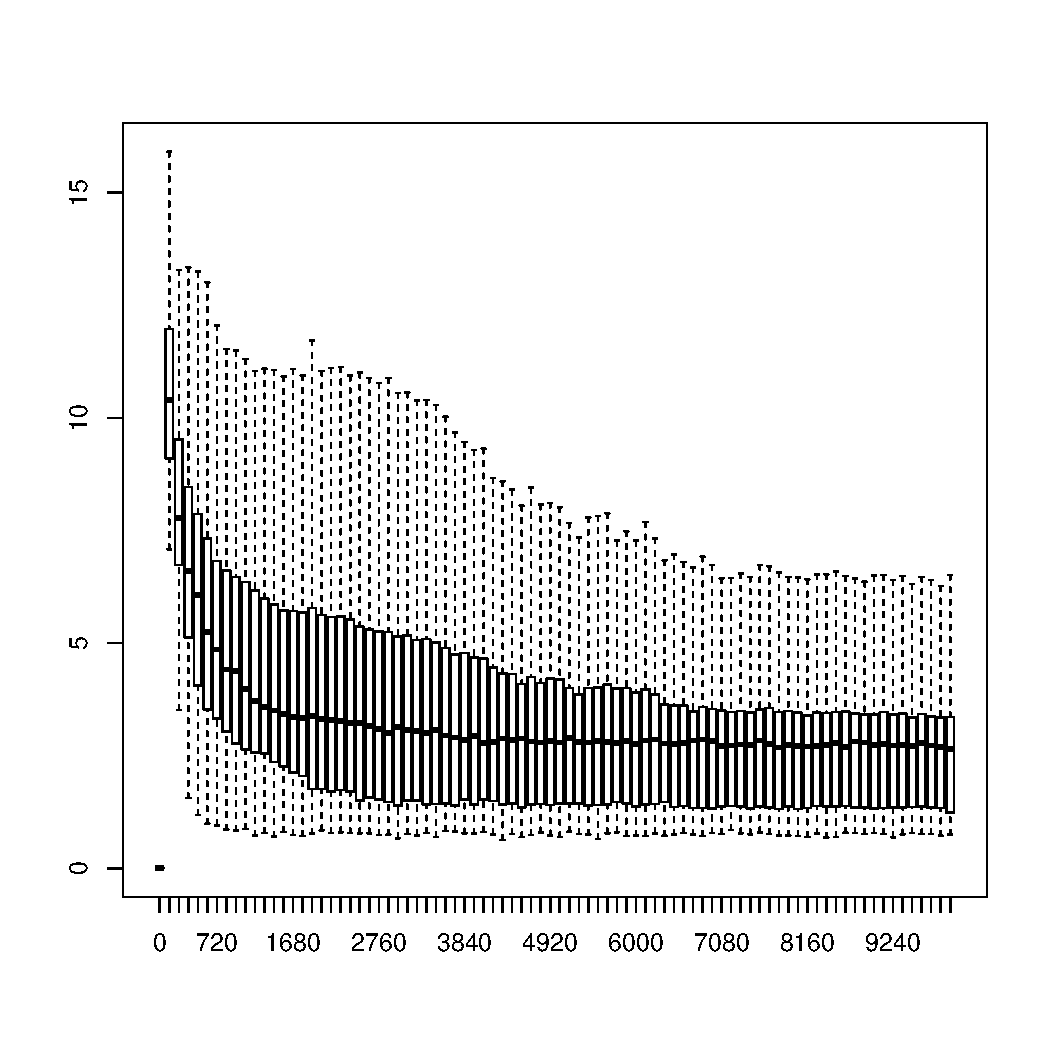
\includegraphics[width=5cm]{img/full.pdf}


		    \end{tabular}
		    \caption{Evolution of the score within the two different models for two typical run with 500 agents and 3 goods evolving during 10000 timesteps.}%%
		    \label{fig:scoreEvol}
		\end{figure}

		%    We first compare the impact of different $CulturalTransmission$ mechanism on the distribution of frequencies of traits (the belief about the price of each goods). 
		%    \begin{figure}[H]
		%	\centering
		%	\setlength{\columnseprule}{0pt}
		%	\begin{multicols}{2}
		%	    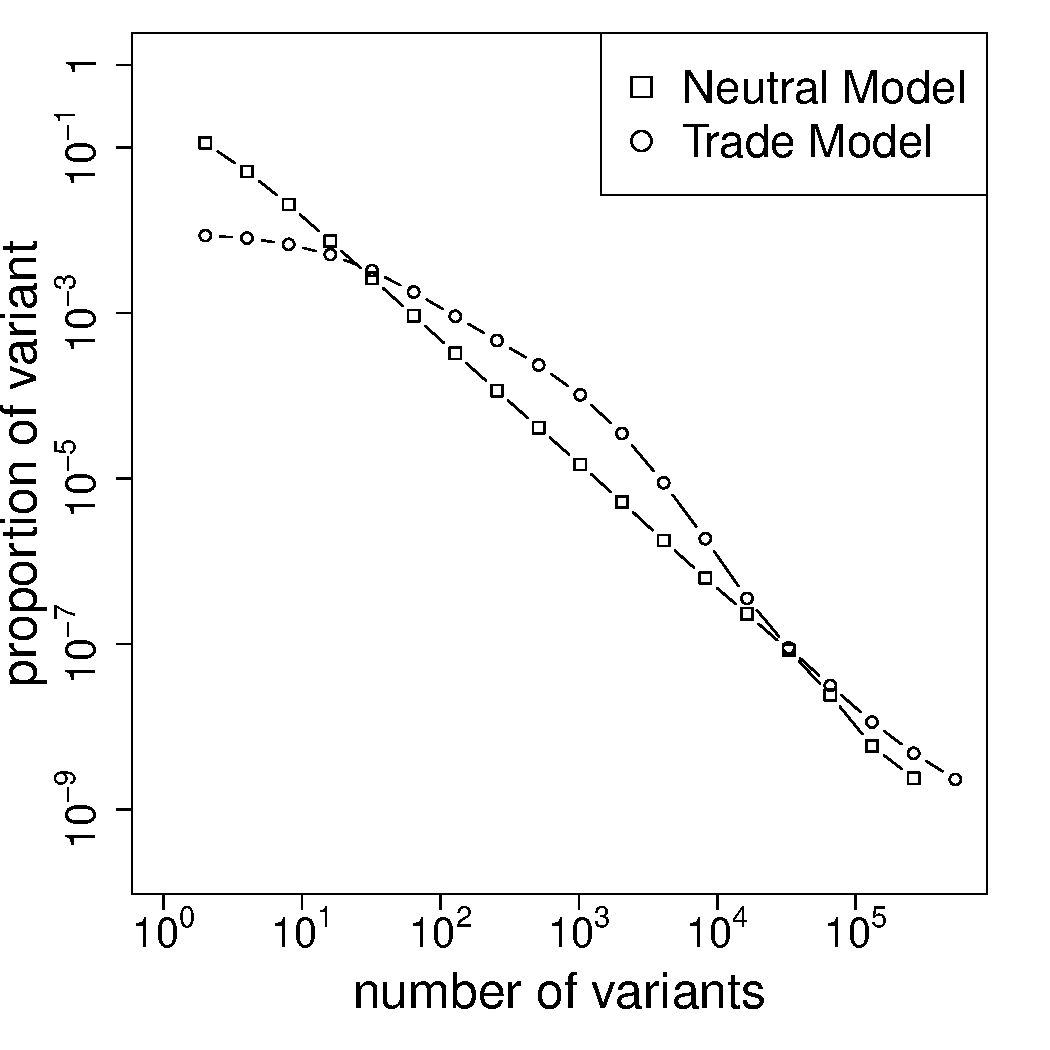
\includegraphics[width=5.2cm]{img/2SetupDistribA.pdf} 
		%	    \caption{Comparaison of the distribution of frequencies between the neutral and the trade model.}
		%	    \label{fig:2setDi}
		%	\end{multicols}
		%    \end{figure}
		%    \vspace{-.8cm}
		%    The figure~\ref{fig:2setDi} shows that when $CulturalTransmission$ is neutral (agents randomly copy prices) the distribution follow the well know power law \cite{bentley_random_2004} but when transmission is not neutral but biased by the economical success of the agents, the power law disappear.

	    }




	    \headerbox{ Cultural Network Topologies}{name=res1,column=1,span=1,row=0}{
		%\begin{multicols}{2}
		    \subsection*{Experimental Setup}

		    \begin{center}
			\huge
			\begin{tabular}{l|ccc}
			    & $D_1$	 	& \dots & $D_n$		\\\hline
			    $A_1$	& $Net_{11}$	& 	& $Net_{1n}$	\\	
			    \dots	&		&\dots	&		\\
			    $A_m$	& $Net_{m1}$	& 	& $Net_{mn}$	\\	
			\end{tabular}
		    \end{center}

		    \begin{center}
			\begin{tabular}{lccc}
			    &$D=0.02$ & $D=0.04$\\
			    $A\approx17$&
			    
\includegraphics[width=2.5cm]{img/g02.pdf}&
			    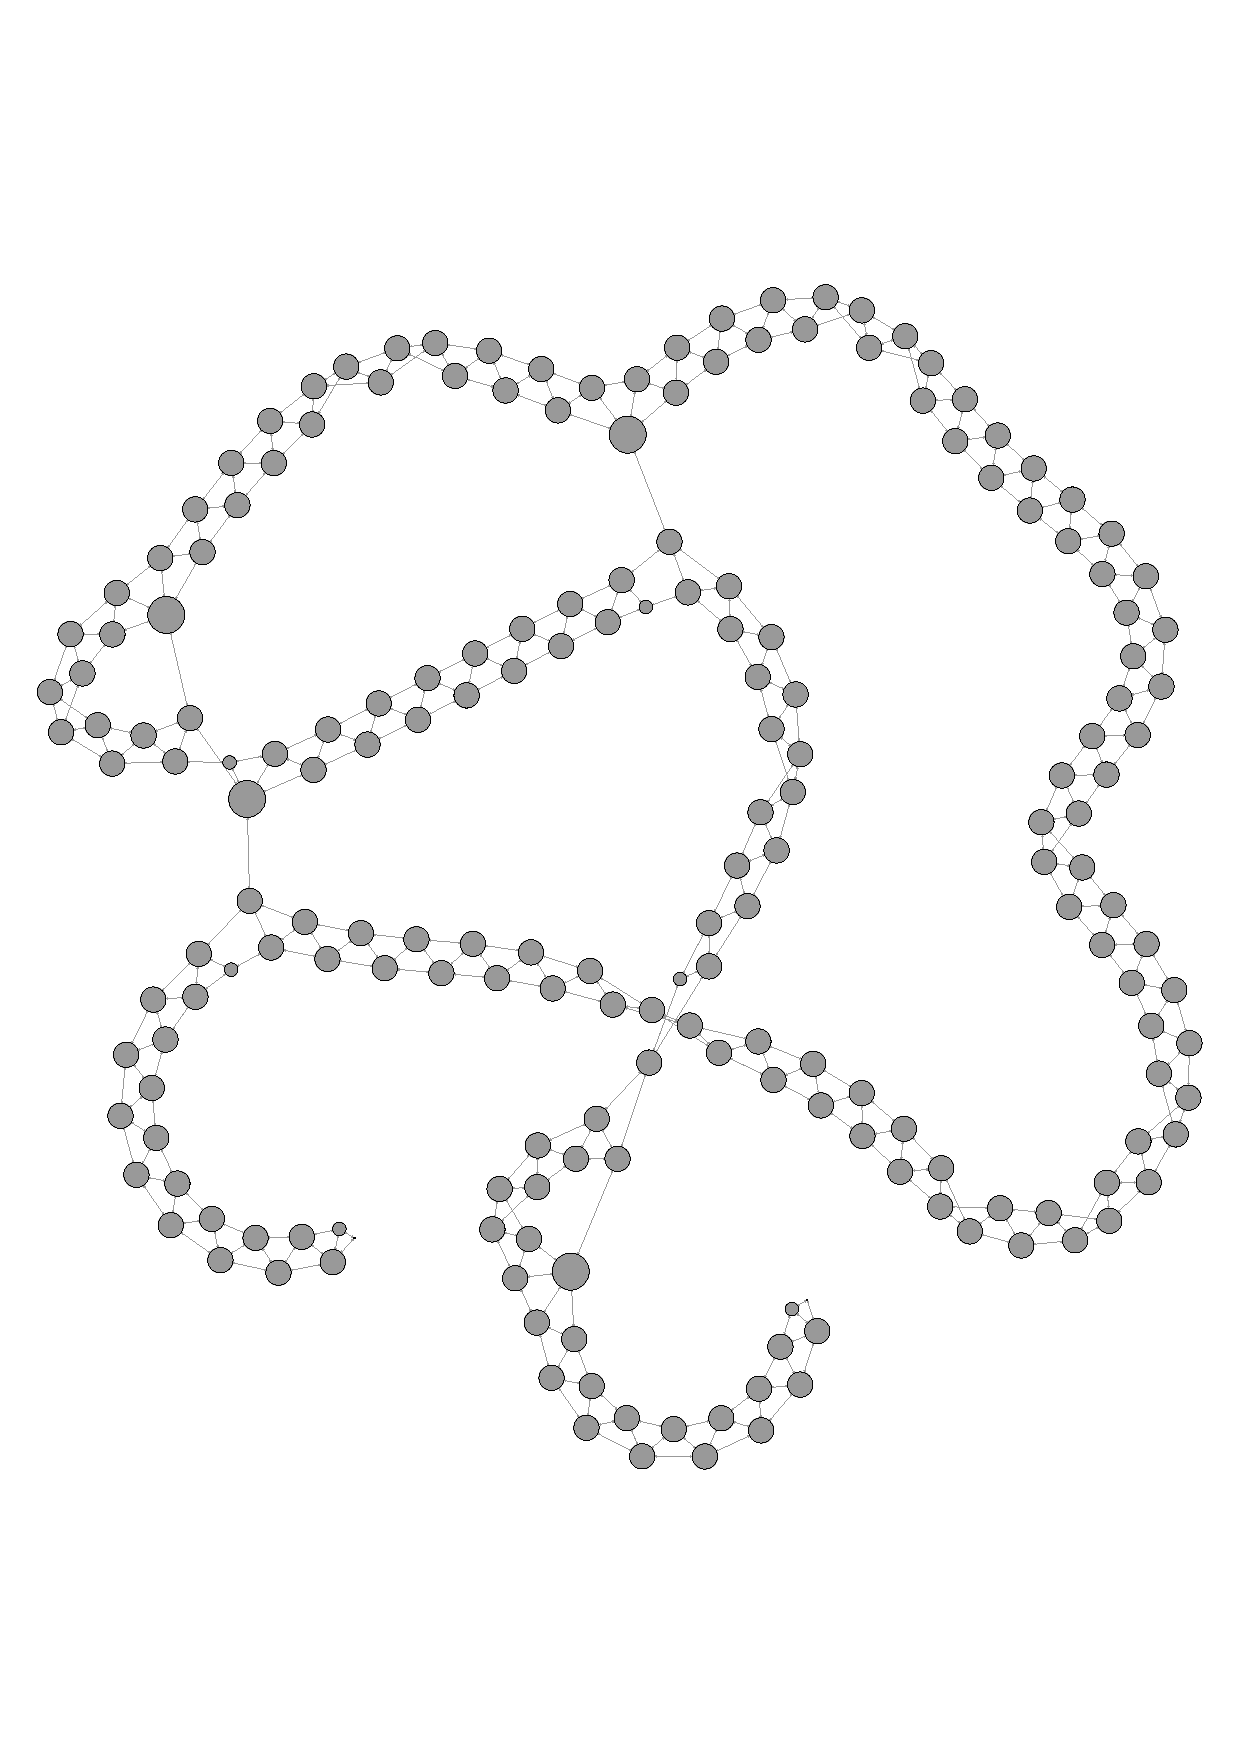
\includegraphics[width=2.5cm]{img/g00.pdf}\\
			    $A\approx4$&
			    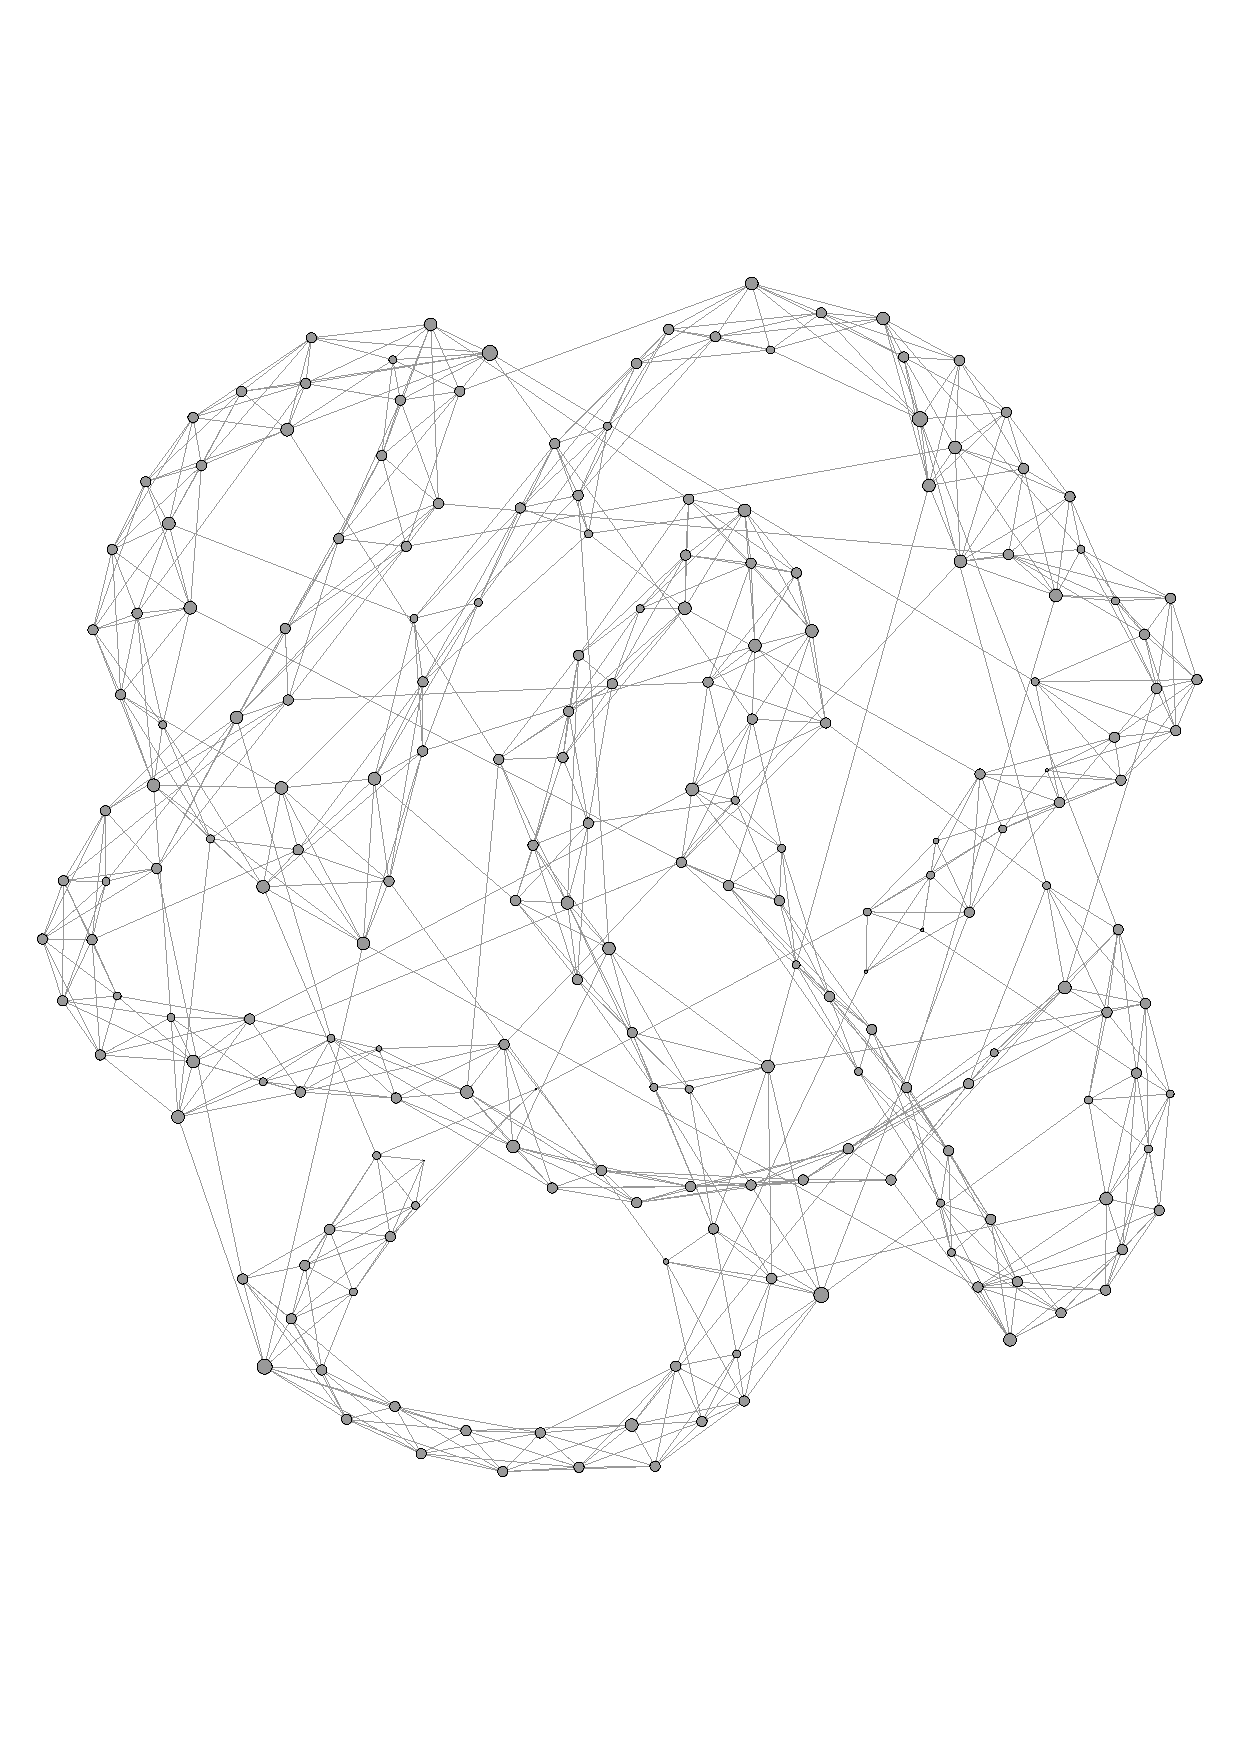
\includegraphics[width=2.5cm]{img/g42.pdf}&
			    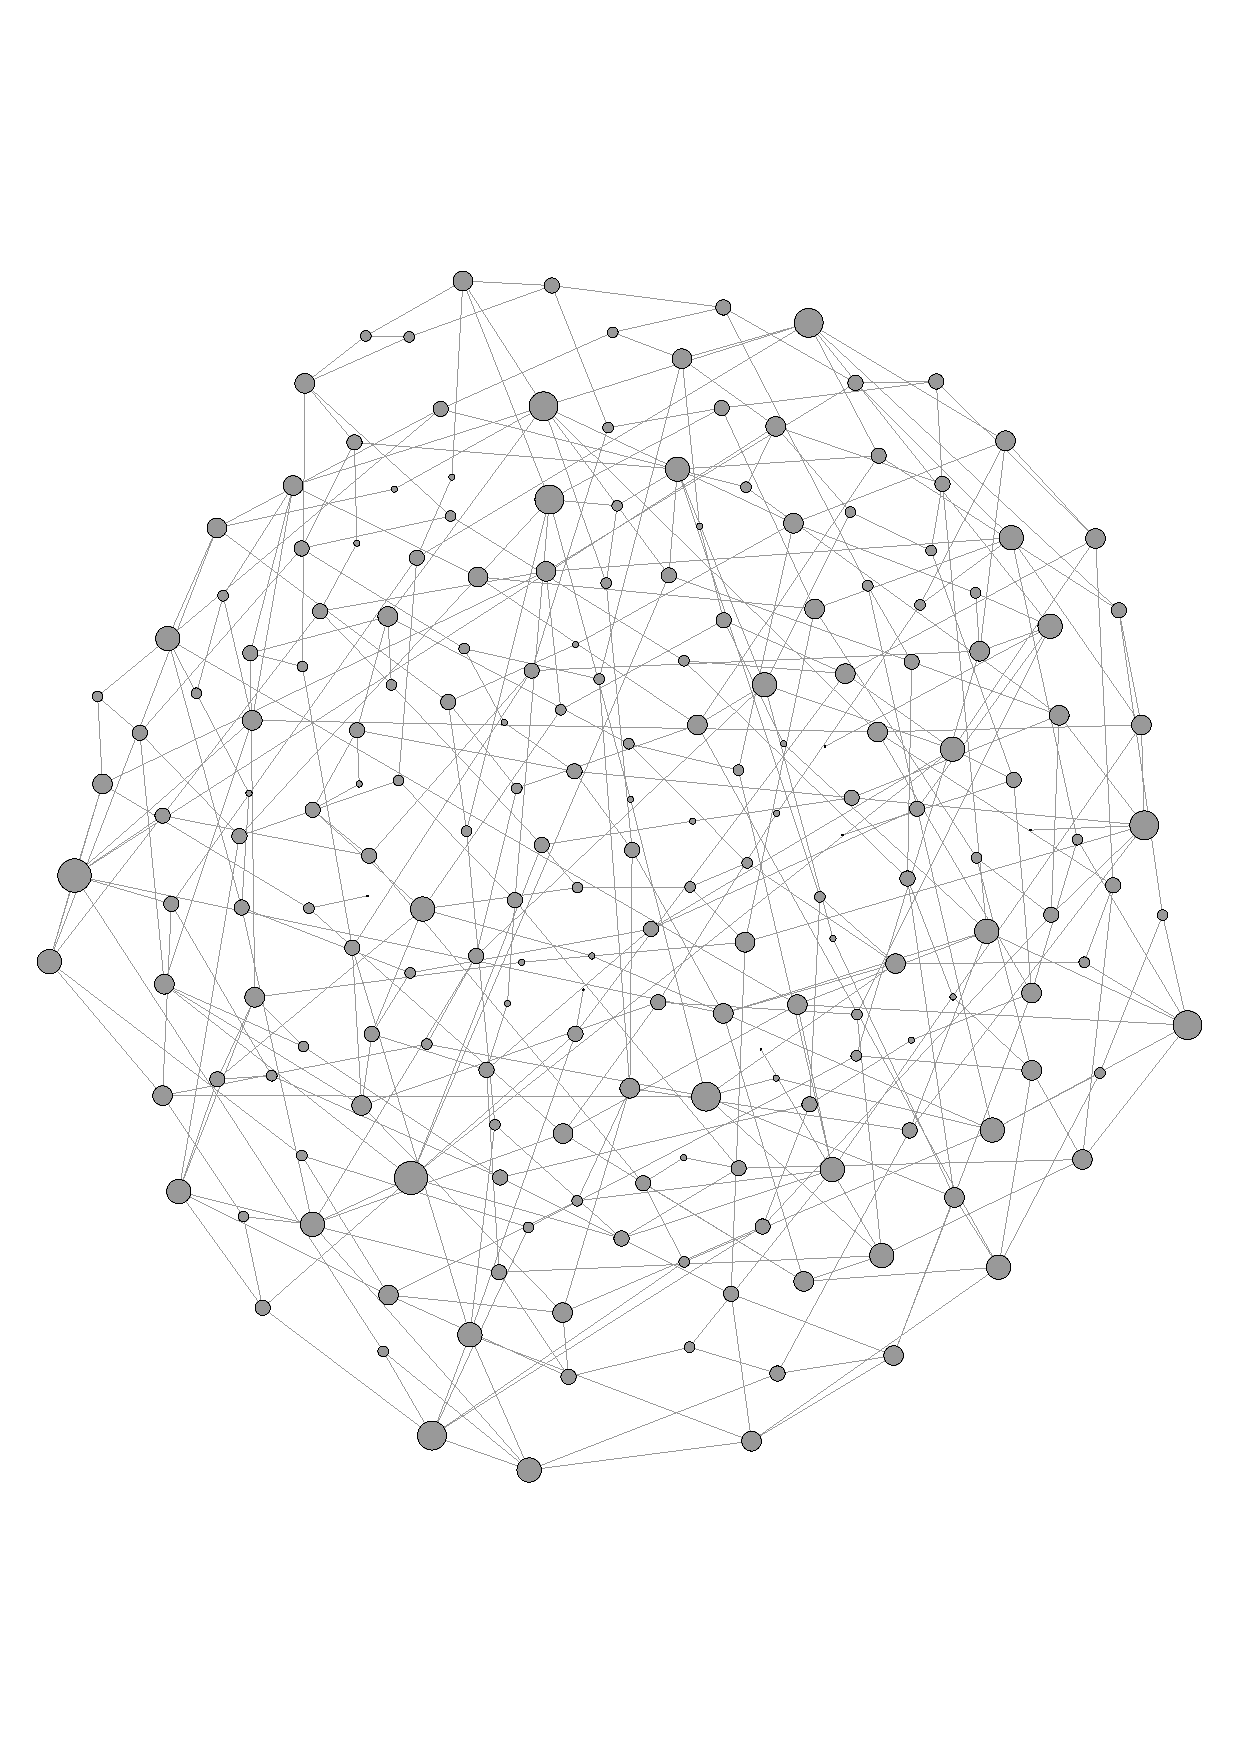
\includegraphics[width=2.5cm]{img/g40.pdf}\\
			\end{tabular}

		    \end{center}


		    As expected when $CulturalTransmission$ is random (i.e., agents modify their belief about the prices randomly), the scores evolve randomly (fig~\ref{fig:scoreEvol}, left) whereas when a non random copy mechanism is used (i.e. agents tend to copy score of successful agents), scores increased toward the maximum score.
		%\end{multicols}
	    \section{Result}
		As shown by the figure~\ref{fig:ratioEvol}, the raise of the score of the agents comes from the fact that the mechanism of $CulturalTransmission$ biased by the economic success of the agents allows them to quickly estimates prices that converge toward their optimal value . Thus it allows them to make more efficient trade and increase their economic success (see also \cite{gintis_emergence_2006}).
		\begin{figure}[H]
		    \center
		    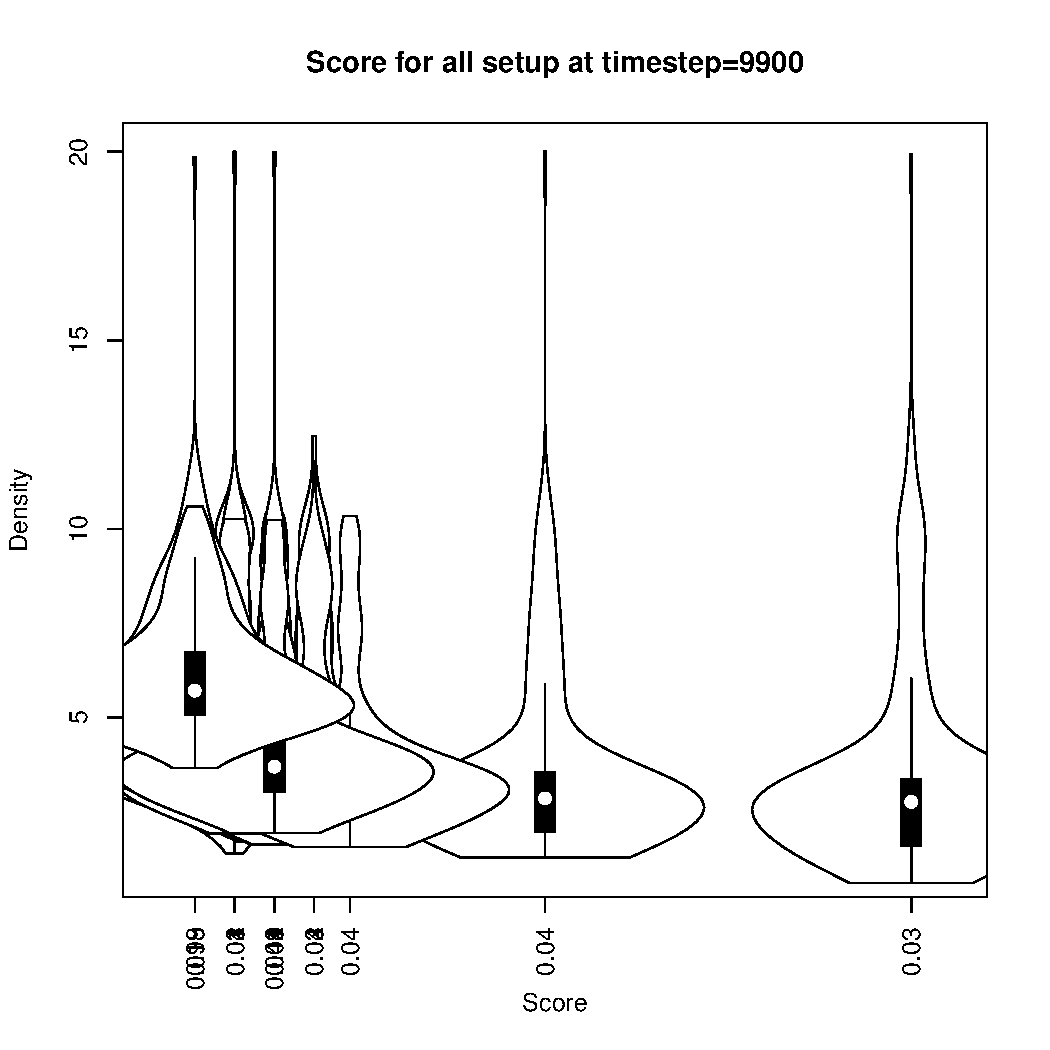
\includegraphics[width=5cm]{img/densVsScore.pdf}
		    \caption{ \small
		    Que guapo es el grande J. Remesal!}
		    \label{fig:ratioEvol}
		\end{figure}



	    }
	    \headerbox{Concluding Remarks}{name=conclusion,column=2,row=0}{
		Integrating cultural and economic dynamics into an evolutionary framework is a good candidate to study such systems. It allows one to study precise mechanisms and to easily test and compare different model of such mechanisms.

		In future works we hope to fruitfully apply that tool to validate, interpret and propose hypotheses about economics and cultural dynamics at work during the Roman Empire.
	    }


	    \headerbox{References}{name=references,column=2,below=conclusion}{
		\scriptsize
		\renewcommand{\refname}{\vspace{-0.5em}}
		\bibliographystyle{unsrt}
		\bibliography{biblio}
	    }
	    \headerbox{Acknowledgements}{name=acknowledgements,column=2,below=references}{
		{\Huge RREMESAL REMESAL REMESAL REMESAL REMESAL REMESAL REMESAL REMESAL REMESAL REMESAL REMESAL REMESAL REMESAL REMESAL REMESAL REMESAL REMESAL REMESAL REMESAL REMESAL REMESAL REMESAL REMESAL REMESAL REMESAL REMESAL REMESAL REMESAL REMESAL REMESAL REMESAL REMESAL REMESAL REMESAL REMESAL REMESAL REMESAL REMESAL REMESAL REMESAL REMESAL REMESAL REMESAL EMESAL REMESAL REMESAL REMESAL REMESAL REMESAL REMESAL REMESAL REMESAL REMESAL REMESAL REMESAL REMESAL REMESAL REMESAL REMESAL REMESAL REMESAL REMESAL REMESAL REMESAL REMESAL REMESAL REMESAL REMESAL REMESAL REMESAL REMESAL REMESAL REMESAL REMESAL REMESAL REMESAL REMESAL REMESAL REMESAL REMESAL REMESAL REMESAL REMESAL REMESAL }
		Funding for this work was provided by the ERC Advanced Grant EPNet (340828).
		\begin{center}
		    
\includegraphics[width=2cm]{logos/bscLogo.jpg}
	%\raisebox{.35\height}{
\includegraphics[width=1cm]{logos/logoSimpast.png}}
		    
\includegraphics[width=1.5cm]{logos/LOGO-ERC.jpg}
		\end{center}
	    } 

	\end{poster}

	\end{document}

